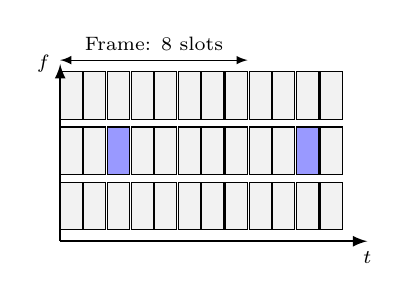
\begin{tikzpicture}[>=latex]
    % Carriers (FDMA) divided into repeating time slots (TDMA)
    \foreach \carrier in {0,1,2} {
        \foreach \slot in {0,...,11} {
            \draw[fill=gray!10] ({0.3*\slot},{0.15+0.7*\carrier}) rectangle ({0.28+0.3*\slot},{0.75+0.7*\carrier});
        }
    }
    % One user occupies the same slot in every frame
    \foreach \slot in {2,10} {
        \draw[fill=blue!40] ({0.3*\slot},0.85) rectangle ({0.28+0.3*\slot},1.45);
    }
    \draw[<->] (0,2.3) -- (2.38,2.3) node[midway, above, font=\scriptsize] {Frame: 8 slots};
    \draw[->, thick] (0,0) -- (3.9,0) node[below, font=\scriptsize] {$t$};
    \draw[->, thick] (0,0) -- (0,2.25) node[left, font=\scriptsize] {$f$};
\end{tikzpicture}
